\subsection{Logistic regression}

As first approach we tried to model our target using logistic regression.

First of all we fitted a model using all the features, that we will name model A, and the result is displayed in \Fig~\ref{fig:LRAllSum}. The model suggested that many variables are not significantly different from zero, with respect to an $\alpha = 0.01$. Therefore we removed those variables and fitted the model again getting the one in \Fig~\ref{fig:LRImpSum}, that we will name model B.

\begin{figure}[h]
	\begin{subfigure}{.6\textwidth}
		\centering
		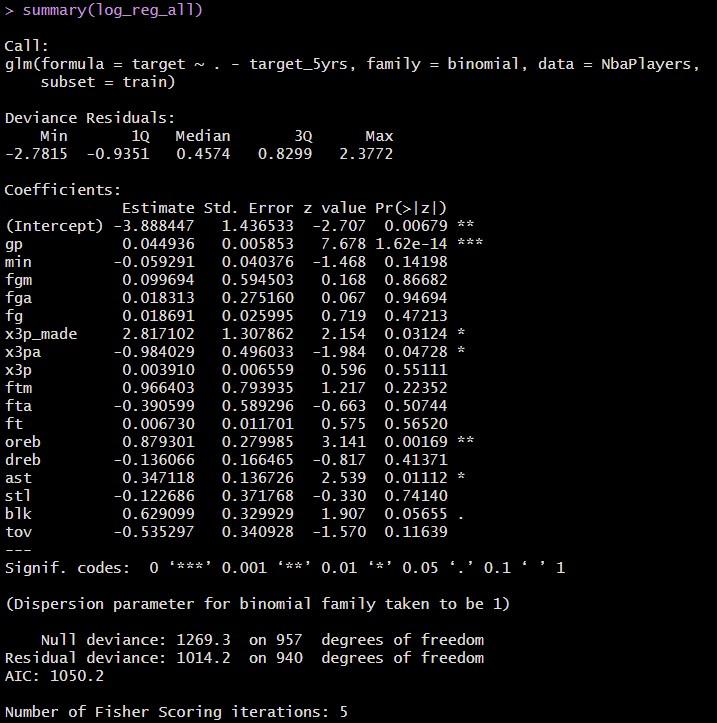
\includegraphics[width=0.7\linewidth]{ImageFiles/Classification/LogReg/log_reg_tt_all_summary}
		\caption{Logistic regression with all features.}
		\label{fig:LRAllSum}
	\end{subfigure}
	\begin{subfigure}{.6\textwidth}
		\centering
		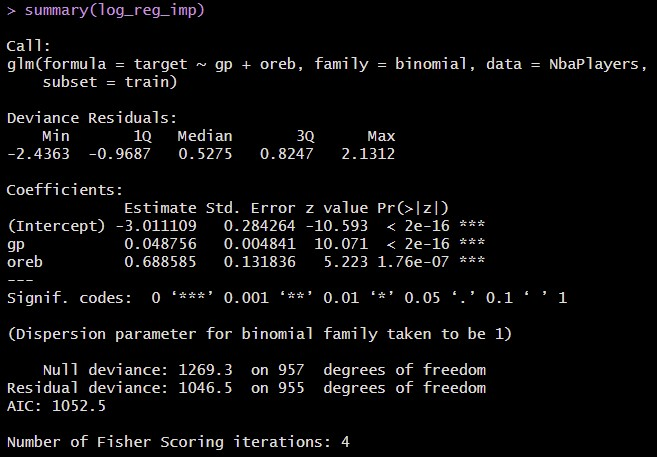
\includegraphics[width=0.8\linewidth]{ImageFiles/Classification/LogReg/log_reg_tt_imp_summary}
		\caption{Logistic regression with only significant features.}
		\label{fig:LRImpSum}
	\end{subfigure}
	\caption{Logistic regression model summary.}
	\label{fig:LRSum}
\end{figure}

It can be observed that there is no significant change in performance. When all variables are used, the accuracy is $70\%$, compared to $67.5\%$ in the second case. Furthermore, the AIC coefficient changes from 1052.5 to 1050.2, which could be considered almost the same. 

\Fig~\ref{fig:CM} shows the confusion matrices for the two models. In general, both models tend to perform slightly better in predicting the ``yes'' class.

\begin{figure}[h]
	\begin{subfigure}{.6\textwidth}
		\centering
		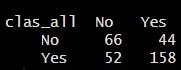
\includegraphics[width=0.7\linewidth]{ImageFiles/Classification/LogReg/log_reg_tt_all_pred_table}
		\caption{Confusion matrix of model A.}
		\label{fig:CMA}
	\end{subfigure}
	\begin{subfigure}{.6\textwidth}
		\centering
		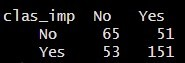
\includegraphics[width=0.7\linewidth]{ImageFiles/Classification/LogReg/log_reg_tt_imp_pred_table}
		\caption{Confusion matrix of model B.}
		\label{fig:CMB}
	\end{subfigure}
	\caption{Confusion matrices.}
	\label{fig:CM}
\end{figure}

Another comparison made between the two models concerns the predicted probabilities, as values close to 0.5 suggest high uncertainty of the model. Histograms showing the predicted values distribution for both models are presented in \Fig~\ref{fig:ProbPred}. From this point of view, model B appears to perform better, but in general, the two models exhibit the same behavior.

\begin{figure}[h]
	\begin{subfigure}{.6\textwidth}
		\centering
		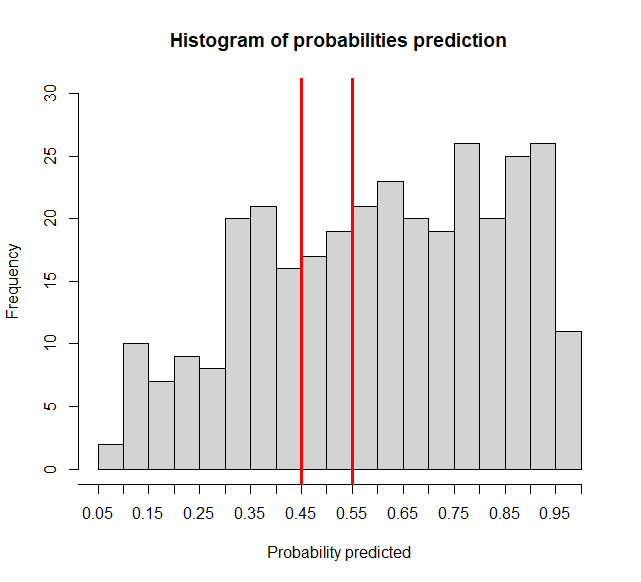
\includegraphics[width=0.7\linewidth]{ImageFiles/Classification/LogReg/probability_pred_all}
		\caption{Probabilities predicted by model A.}
		\label{fig:ProbPredA}
	\end{subfigure}
	\begin{subfigure}{.6\textwidth}
		\centering
		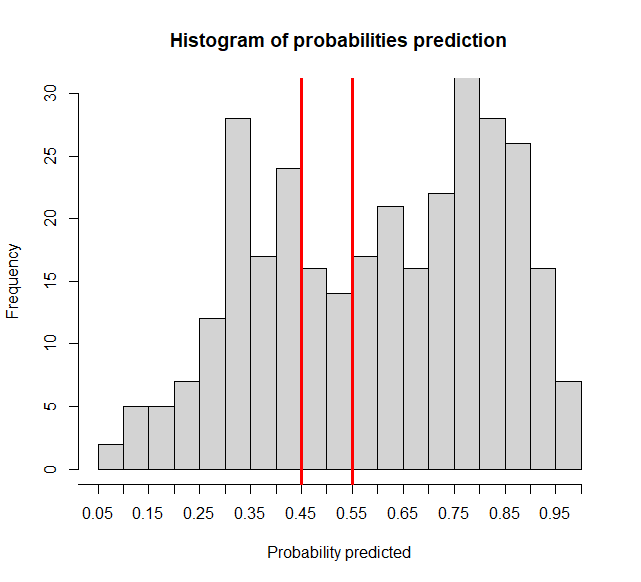
\includegraphics[width=0.7\linewidth]{ImageFiles/Classification/LogReg/probability_pred_imp}
		\caption{Probabilities predicted by model B.}
		\label{fig:ProbPredB}
	\end{subfigure}
	\caption{Probabilities predicted.}
	\label{fig:ProbPred}
\end{figure}

The model fitted using only the important variables shows the same performance as the first one, but it uses variables, making it a better choice.

\vspace{0.2cm}
\textbf{Subset selection}

After the initial analysis, we attempted variable selection using subset selection algorithms, specifically the forward stepwise and backward stepwise methods were applied. 

The results obtained are presented in \Fig~\ref{fig:LRSSSum}. The forward stepwise method resulted in a model that essentially includes all the variables. In contrast, the backward stepwise method resulted in a model with 11 variables, but 7 of them are not significantly different from zero with respect to $a\alpha = 0.01$. The model achieved an $AIC = 1040.4$ and accuracy of $70\%$. The performances are again quiet similar, the AIC coefficient is slightly better for the backward model.

\begin{figure}[h]
	\begin{subfigure}{.6\textwidth}
		\centering
		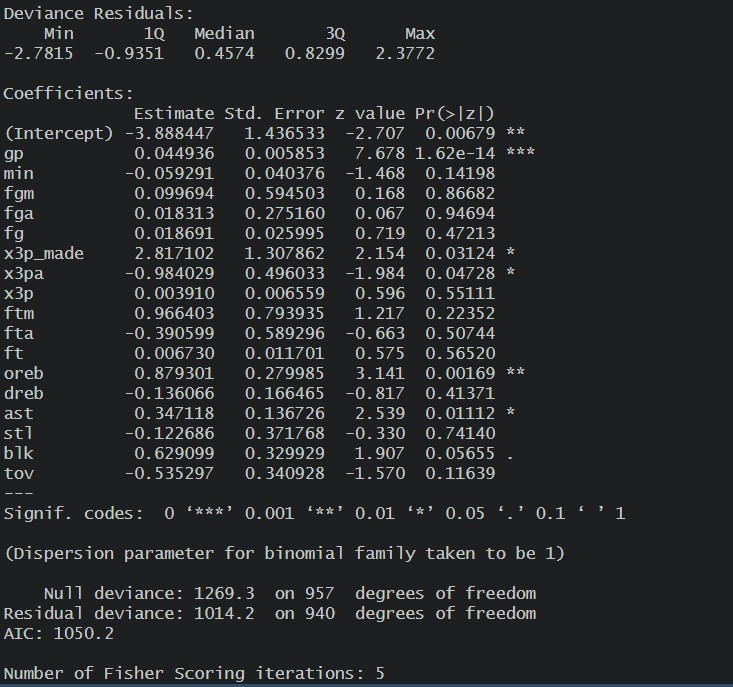
\includegraphics[width=0.7\linewidth]{ImageFiles/Classification/LogReg/lr_fss_summary}
		\caption{Logistic regression with forward stepwise.}
		\label{fig:LRFSSSum}
	\end{subfigure}
	\begin{subfigure}{.6\textwidth}
		\centering
		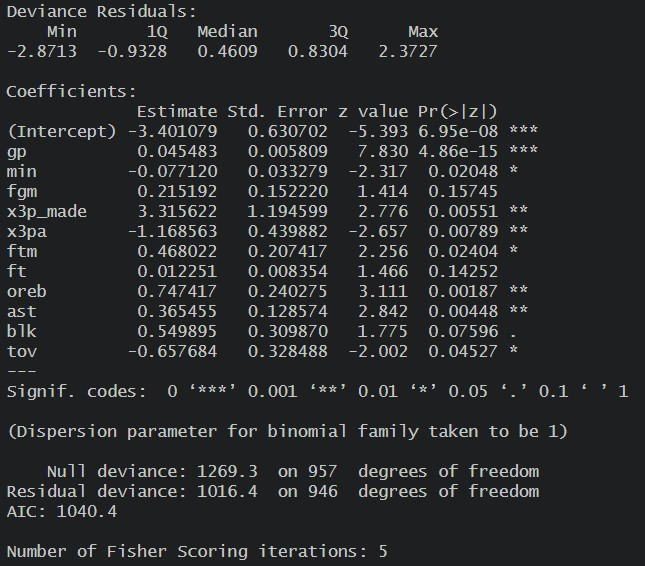
\includegraphics[width=0.7\linewidth]{ImageFiles/Classification/LogReg/lr_bss_summary}
		\caption{Logistic regression with backward stepwise.}
		\label{fig:LRBSSSum}
	\end{subfigure}
	\caption{Logistic regression models with subset selection.}
	\label{fig:LRSSSum}
\end{figure}

Since the forward model includes all the variables, its analysis is identical to the first one.

After removing the non-significant variables from the backward model, we obtained the same model as in the previous analysis, which we referred to as model B. 

This confirms our results, suggesting that the model with only ``GP'' and ``OREB'' explains in a good way the target. 

\vspace{0.2cm}
\textbf{Conclusions and Observations}

In general, regardless of the variables included, logistic regression is able to achieve an accuracy around $70\%$. Therefore, it may be better to explore other classification methods to potentially improve the model's performances.

However, the logistic regression model obtained suggests that a good trade-off between model simplicity and performances can be achieved with two variables. In particular:

\begin{itemize}
	\item The inclusion of ``GP'' was expected, as it makes sense that players who play more games will have a longer career. The second feature, on the other hand, is not really intuitive and revealed a new characteristic about the data.
	\item In general, all models perform better at predicting the ``yes'' class instead of the ``no'' class, but this can be traced back to the composition of the dataset, which includes more ``yes'' samples than ``no''.
\end{itemize}

The performances achieved with logistic regression are limited, therefore other classification techniques will be explored in the following sections.
